%\section{Selection Cuts for eleTau Channel}
\section{\texorpdfstring{Selection cuts for \leptonTau channel}{Selection cuts for lepton-tau channel}}
\label{sect:eleTauCuts}

In the \leptonTau final states, events are selected when one electron(muon) with \PT $>$ 25 (20) \GeV and $|\eta|$ $<$ 2.1 and at least 
one oppositely charged \Tau with \PT $>$ 20 \GeV and $|\eta|$ $<$ 2.1 exist. $I_{\Tau}$ of the hadronic tau must be less than 0.8 \GeV.
In the case of more than one pair, the pair that maximizes the sum $\PT^{\Tau} + \PT^{Lep}$ is selected.
Vetoing the second lepton with \PT $>$ 10 \GeV and loose isolation criteria helps to suppress the $Z\rightarrow \mu\mu, ee$ background.

After requesting two opposite sign leptons in the events, a loose cut on \MET $>$ 30 \GeV is applied to supress QCD multijet events. 
As there is no b-quark in the signal, rejecting events with one or more b-tagged jets helps a lot in reducing \ttbar and $W+b$ backgrounds.

To reject QCD low mass resonances, the invariant mass of the lepton and \Tau is requested to be greater than 15 \GeV. 
Another cut on the invariant mass of the di-lepton system is applied to remove the peak of the $\Z$jets events. 
It has been found that the visible mass of the $Z\to\tau\tau\to\,e/\mu +\Tau$ moves to 60 $\pm$ 15 \GeV due to 
mis-reconstruction of the energy of the hadronic $\tau$ and also the missing energy due to the decay of the $\tau$ to leptons. 
So the events with the invariant mass of lepton \Tau in the window of [45, 75] are excluded from the analysis (\Z-veto). 
The minimum angle in the transverse plane between the \MET and the jets with \PT $>$ 40 \GeV and $|\eta| <$ 5 
is asked to be greater than 1. This cut and a soft cut on \mttwo ($>$ 40 \GeV) kills the bulk of the QCD events 
to get rid of related uncertainities due to mis-reconstruction of the QCD events. 
%As it has mentioned above, the signal events are expected to have high $MT2$ values due to the intrinsic \MET.
%The cut flow tables for the electron/$\mu$ $\,+\tau$ pre-selections are shown in tables .... and ... respectively. The distribution of the $p_{T}$ of the $\tau$ and $MET$ in the pre-selected events in both channels are shown in FIGS ... . The good agreement between data and MC confirms that the needed correction factors are considrred carefully.

Similar to the \tauTau channel, a hard cut on \mttwo ($>$ 90 \GeV) is useful to supress different SM backgrounds, especially $W$jet events.
Such a high cut on the \mttwo increases the sensitivity of the study to signal events with high mass difference. The \Tau transverse mass (\tauMT)
is found to be a good discriminator to further suppress the $W$-jets events which is the main background in this step. 
Opposite to the \tauTau channel, the events with \mttwo $<$ 90 \GeV are not useful in \leptonTau channels and they can not add any power to 
the final exclusion. The bins for $e\Tau$ and $\mu\Tau$ channels are defined by the following selections:
\begin{itemize}
\item \mttwo $>$ 90 \GeV.
\item \tauMT $>$ 200 \GeV; 
\end{itemize}

 The composition of the backgrounds and number of remaining signals for both channels can be found in the table \ref{tbl:yieldsLepTau}.

\begin{table}[!Hhtb]
\begin{center}
%\begin{tiny}
\begin{tabular}{lccccccccc}
\hline
\hline
  & SUSY(380,1) & QCD & W & ZX & Top & WW & Higgs & MC & Data \\
\hline
\hline
e\Tau & 2.14  & 0 & 1.29 & 0.38 & 0.02 & 0.05 & 0.06 & 1.79$\pm$0.63 & 3 \\
\hline
$\mu\hadtau$& 2.09 & $<$16.78 & 0.79 & 0.28 & $<$0.61 & 0.34 & 0.05 & 1.46$\pm$.49 & 5 \\
%QCD 70.87 +- 34.49
%Top 1.15 +- 0.84
\hline
\hline
\end{tabular}
\caption{Yields for e\Tau and $\mu\hadtau$ channels. Only statistical uncertainties are reported.When the remaining events from MC are zero, the weight of the events is reported as the upper bound.}
\label{tbl:yieldsLepTau}
%\end{tiny}
\end{center}
\end{table}

Figures \ref{fig:mt2leptontau} and \ref{fig:taumtleptontau} show the \mttwo and \tauMT distributions before applying the cut on \tauMT.
\begin{figure}[!Hhtb]
\centering
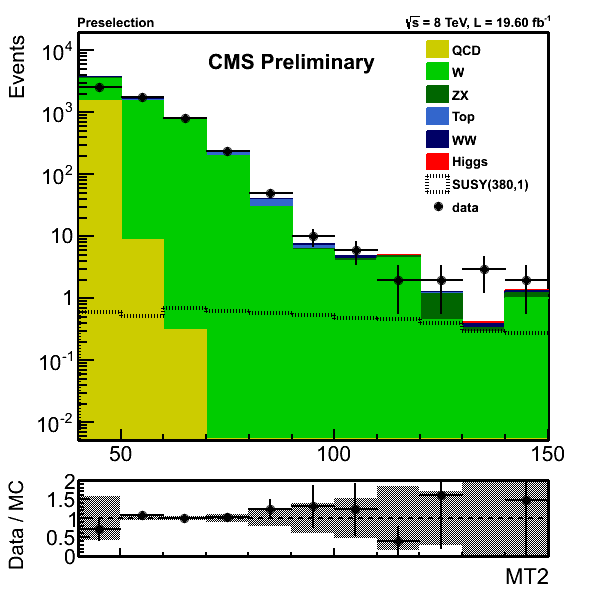
\includegraphics[angle=0,scale=0.35]{SelectionEleTau/MT2.png}
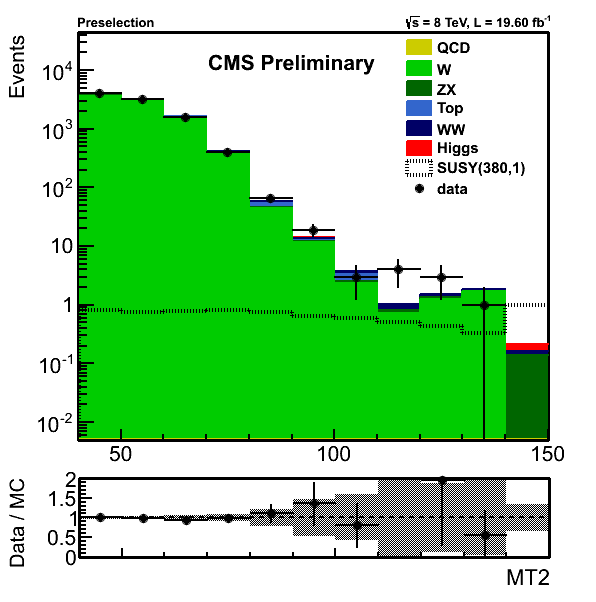
\includegraphics[angle=0,scale=0.35]{SelectionMuTau/MT2_Ratio_Preselection_unBlinded.png}
\caption{\mttwo distribution of preselected events in (Left) $e\hadtau$ and (Right) $\mu\hadtau$ channels.}
\label{fig:mt2leptontau}
\end{figure}


\begin{figure}[!Hhtb]
\centering
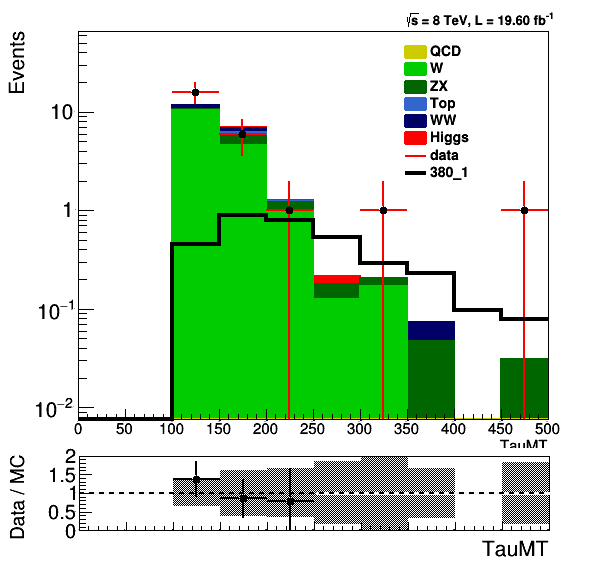
\includegraphics[angle=0,scale=0.35]{SelectionEleTau/TauMT.png}
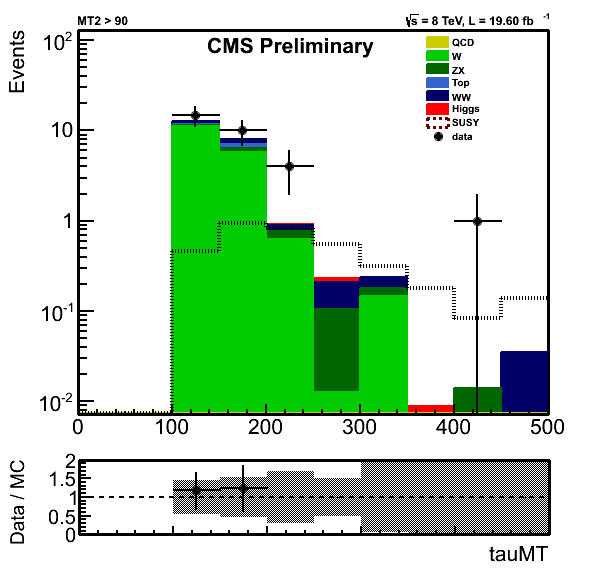
\includegraphics[angle=0,scale=0.35]{SelectionMuTau/tauMT_Ratio_MT2gt90_unBlinded.png}
\caption{\tauMT distribution for events with $\mttwo>90\GeV$ in (Left) $e\hadtau$ and (Right) $\mu\hadtau$ channels.}
\label{fig:taumtleptontau}
\end{figure}
%Opposite to the $\Tau\Tau$ channel, the events with $\mttwo<90 \GeV$ are not useful in $\ell\Tau$ channels because of the contamination of
%the Wjets events. It was investigated if increasing the \pt of the objects can increase the sensitivity in this bin, but no improvement was seen.

